%% Aide-mémoire
\documentclass[10pt, french]{article}
%% -----------------------------
%% Préambule
%% -----------------------------
\usepackage{xcolor}
\usepackage{bbding}
\usepackage{pifont}
\usepackage{tikz}
\def\BackgroundColor{white}
\def\SectionColor{teal!90!black}
\def\SubSectionColor{teal!45!black}
% !TEX encoding = UTF-8 Unicode
% LaTeX Preamble for cheatsheet
% Author : Gabriel Crépeault-Cauchon

% HOW-TO : copy-paste this file in the same directory as your .tex file, and add in your preamble the next command right after you have specified your documentclass :
% \input{preamble-cheatsht.tex}
% ---------------------------------------------
% ---------------------------------------------

% Extra note : this preamble creates document that are meant to be used inside the multicols environment. See the documentation on internet for further information.

%% -----------------------------
%% Encoding packages
%% -----------------------------
\usepackage[utf8]{inputenc}
\usepackage[T1]{fontenc}
\usepackage{babel}
\usepackage{lmodern}

%% -----------------------------
%% Variable definition (change these values)
%% -----------------------------
\def\cours{Analyse probabiliste des risques actuariels}
\def\sigle{ACT-1002}
\def\session{H2017}
\def\auteur{Gabriel Crépeault-Cauchon}
\def\BackgroundColor{white}
\def\SectionColor{teal!50!black}
\def\SubSectionColor{teal!20!black}

%% -----------------------------
%% Margin and layout
%% -----------------------------
% Determine the margin for cheatsheet
\usepackage[landscape, hmargin=1cm, vmargin=1.7cm]{geometry}
\usepackage{multicol}

% Remove automatic indentation after section/subsection title.
\setlength{\parindent}{0cm}

% Save space in cheatsheet by removing space between align environment and normal text.
\usepackage{etoolbox}
\newcommand{\zerodisplayskips}{%
  \setlength{\abovedisplayskip}{0pt}%
  \setlength{\belowdisplayskip}{0pt}%
  \setlength{\abovedisplayshortskip}{0pt}%
  \setlength{\belowdisplayshortskip}{0pt}}
\appto{\normalsize}{\zerodisplayskips}
\appto{\small}{\zerodisplayskips}
\appto{\footnotesize}{\zerodisplayskips}

%% -----------------------------
%% URL and links
%% -----------------------------
\usepackage{hyperref}
\hypersetup{colorlinks = true, urlcolor = gray!70!white, linkcolor = black}

%% -----------------------------
%% Document policy (uncomment only one)
%% -----------------------------
%	\usepackage{concrete}
	\usepackage{mathpazo}
%	\usepackage{frcursive} %% permet d'écrire en lettres attachées
%	\usepackage{aeguill}
%	\usepackage{mathptmx}
%	\usepackage{fourier}

%% -----------------------------
%% Math configuration
%% -----------------------------
\usepackage[fleqn]{amsmath}
\usepackage{amsthm,amssymb,latexsym,amsfonts}
\usepackage{empheq}
\usepackage{numprint}

% Mathematics shortcut
\newcommand{\reels}{\mathbb{R}}
\newcommand{\entiers}{\mathbb{Z}}
\newcommand{\naturels}{\mathbb{N}}
\newcommand{\eval}{\biggr \rvert}
\usepackage{cancel}
\newcommand{\derivee}[1]{\frac{\partial}{\partial #1}}
\newcommand{\prob}[1]{\Pr \left( #1 \right)}
\newcommand{\esp}[1]{\mathrm{E} \left[ #1 \right]} % espérance
\newcommand{\variance}[1]{\mathrm{Var} \left( #1   \right)}
\newcommand{\covar}[1]{\mathrm{Cov} \left( #1   \right)}
\newcommand{\laplace}{\mathcal{L}}

% To indicate equation number on a specific line in align environment
\newcommand\numberthis{\addtocounter{equation}{1}\tag{\theequation}}

% Actuarial notation package
\usepackage{actuarialsymbol}
\usepackage{actuarialangle}

% Matricial anotation for math symbols (\bm{•})
\usepackage{bm}
% matricial notation variable (bold style)
\newcommand{\matr}[1]{\mathbf{#1}}



%% -----------------------------
%% tcolorbox configuration
%% -----------------------------
\usepackage{tcolorbox}
\tcbuselibrary{xparse}
\tcbuselibrary{breakable}

%% Définition boite pour définition
\DeclareTColorBox{definition}{ o }% #1 parameter
{colframe=blue!60!green,colback=blue!5!white, % color of the box
breakable, pad at break*=0mm, % to split the box
title = {#1},
after title = {\large \hfill \faBook}
}

%% -----------------------------
%% Graphics and pictures
%% -----------------------------
\usepackage{graphicx}
\usepackage{pict2e}

%% -----------------------------
%% insert pdf pages into document
%% -----------------------------
\usepackage{pdfpages}

%% -----------------------------
%% Color configuration
%% -----------------------------
\usepackage{color, soulutf8, colortbl}

% usefull shortcut for colored text
\newcommand{\orange}{\textcolor{orange}}
\newcommand{\red}{\textcolor{red}}
\newcommand{\cyan}{\textcolor{cyan}}
\newcommand{\blue}{\textcolor{blue}}
\newcommand{\green}{\textcolor{green}}
\newcommand{\purple}{\textcolor{magenta}}
\newcommand{\yellow}{\textcolor{yellow}}


%% -----------------------------
%% Enumerate environment configuration
%% -----------------------------
% Custum enumerate & itemize Package
\usepackage{enumitem}
% French Setup for itemize function
\frenchbsetup{StandardItemLabels=true}
% Change default label for itemize
\renewcommand{\labelitemi}{\faAngleRight}

%% -----------------------------
%% Tabular column type configuration
%% -----------------------------
\newcolumntype{C}{>{$}c<{$}} % math-mode version of "l" column type
\newcolumntype{L}{>{$}l<{$}} % math-mode version of "l" column type
\newcolumntype{R}{>{$}r<{$}} % math-mode version of "l" column type
\newcolumntype{f}{>{\columncolor{green!20!white}}p{1cm}}
% configuration to force a line break within a single cell
\usepackage{makecell}



%% -----------------------------
%% Fontawesome for special symbols
%% -----------------------------
\usepackage{fontawesome}

%% -----------------------------
%% Section Font customization
%% -----------------------------
\usepackage{sectsty}
\sectionfont{\color{\SectionColor}}
\subsectionfont{\color{\SubSectionColor}}

%% -----------------------------
%% Footer/Header Customization
%% -----------------------------
\usepackage{lastpage}
\usepackage{fancyhdr}
\usepackage{titling}
\pagestyle{fancy}
% Header
\fancyhead{} 	% Reset
\fancyhead[L]{Aide-mémoire pour~ \cours ~(\textbf{\sigle})}
\fancyhead[R]{\auteur}

% Footer
\fancyfoot{}		% Reset
\fancyfoot[R]{\thepage ~de~ \pageref{LastPage}}
\fancyfoot[L]{\href{https://github.com/gabrielcrepeault/latex-template}{\faGithub \ gabrielcrepeault/latex-template}}

% page background color
\pagecolor{\BackgroundColor}






%% END OF PREAMBLE
% ---------------------------------------------
% ---------------------------------------------

\title{GRF-II \\ Document d'étude}
\author{Nicholas Langevin}
%% -----------------------------
%% Début du document
%% -----------------------------
\begin{document}

% Pour limiter le nombre de page, je met en commentaire la page couverture
% % PAGE COUVERTURE DE L'AIDE-MÉMOIRE
\maketitle 
\vspace{50px}
\begin{center}
\begin{minipage}[c]{7.5cm}
    \begin{itemize}
        \LARGE
        \item[\color{black}\ding{235}] Les produits dérivés 
        \item[\color{black}  \ding{235}] Forwards et autres options
        \item[\color{purple} \ding{235}] Stratégies
        \item[\color{orange} \ding{235}] Forwards et Futures
        % \item[\color{red}    \ding{235}] Statistics
        % \item[\color{blue}   \ding{235}] Extended Linear Model
        % \item[\color{green}  \ding{235}] Time Series      
    \end{itemize}
\end{minipage}
\end{center}
% \newpage

\small
\begin{multicols*}{2} % Nombre de colonnes (peut être changé plus tard.)

\section{Introduction aux produits dérivés}
\paragraph{Produits dérivés} Contrat entre 2 parties qui fixe les flux financiers futurs fondé sur ceux de \underline{l'actif sous-jacent} $S$.

\subsection*{Étapes d'une transaction}
\begin{enumerate}
\item l'acheteur et le vendeur se trouve (sur un marché quelquonque)
\item on définit les obligations de chaques parties (\textit{i.e. actif à livrer, date d'échéance, prix, etc.}. \textbf{Note : il y a souvent un intermédiaire (\textit{clearing house}) qui intervient.}
\item La transaction a lieu et les obligations sont remplies par chaque parties
\item Les registres de propriétés sont mis à jour.
\end{enumerate}

\paragraph{Transaction gré-à-gré} transaction sans intermédiaire ou à l'extérieur de la bourse. Plusieurs raisons peuvent justifier ce type de transaction  :
\begin{itemize}
\item Ce sont souvent de grosses transaction. On peut donc économiser sur les frais de transaction.
\item On peut combiner (sur une même transaction) plusieurs micro-transaction et plusieurs types d'actifs.
\end{itemize}

\paragraph{Valeur notionelle} \hl{définition exacte à valider}

\paragraph{Origine des marchés de produits dérivés} Après 1971, le président Nixon a vouli défaire le standard de l'or (qui a causé de l'hyperinflation dans plusieurs pays) pour plutôt laisser le libre-marché fixer la valeur des devise de chaque pays.

\paragraph{Rôle des marchés financiers} Partage du risque et diversification des risques.

\paragraph{Utilité des produits dérivés}
\begin{itemize}
\item Gestion des risques
\item Spéculation
\item Réduction des frais de transaction
\item Arbitrage réglementaire
\end{itemize}

\paragraph{Bid-Ask Spread} Correspond à la marge que le teneur de marché (\textit{market maker}) conserve. En l'absence d'arbitrage, on aura $Ask - Bid > 0$
\begin{description}
\item[Ask] prix le plus haut que quelqu'un est prêt à payer pour le sous-jacent
\item[Bid] prix le plus bas que quelqu'un est prêt à payer pour le sous-jacent
\end{description}

\subsection*{Terminologie}
\begin{description}
\item[market order] ordre au marché : on achète et vend selon les prix Bid Ask actuels.
\item[limit order] Ordre limite : on achète le sous-jacent si $Ask < k$ ou on vend le sous-jacent si $Bid > k$.
\item[Stop Loss] ordre de vente stop : on veut limiter sa perte si un sous-jacent perd énormément de valeur. Donc, on va vendre le sous-jacent si $Bid \leq k$.
\item[Long] On se considère en position longue sur le sous-jacent si notre stratégie nous permet de bénéficier d'une \green{hausse} du sous-jacent.
\item[Short] On se considère en position longue sur le sous-jacent si notre stratégie nous permet de bénéficier d'une \red{baisse} du sous-jacent.
\end{description}

\paragraph{Type de risques}
\begin{description}
\item[Risque de défaut] Risque de ne pas être payé. Ce risque peut être réduit avec un dépôt initial en garantie ou une marge de sécurité.
\item[Risque de rareté] Si il est difficile de trouver un acheteur et un vendeur pour le sous-jacent (pas beaucoup de transactions signifie beaucoup de négociations et de variation dans les prix)
\end{description}

\section{Introduction aux Forwards et aux options}
Pour chaque stratégie qu'on voit dans le cours, on peut calculer
\begin{description}
\item[Premium] Il s'agit des cashflow à $t=0$ (si positif, il s'agît d'un coût ; si négatif, il s'agît d'une \textit{compensation}).
\item[Payoff] Valeur à l'échéance $t = T$, i.e. les Cash-flow au temps $t = T$.
\item[Profit] $= Payoff - \text{AV}(Premium)\footnote{AV veut dire \textit{accumulated value}.}$
\end{description}

\paragraph{Quelques définitions}
\begin{description}
\item[$r_f$] taux d'intérêt sans risque. Parfois exprimé comme une force d'intérêt $r$ continue.
\item[$S$] Sous-jacent (peut être une action, une devise, ...)
\item[$S_0$] valeur actuelle du sous-jacent $S$.
\item[$S_T$] valeur du sous-jacent $S$ au temps $t = T$.
\item[$F_{0,T}$] Prix \textit{forward} du sous-jacent au temps $T$, qu'on définit comme
\[F_{0,T} = S_0 (1 + r_f)^{T}\]
\item[$F_{0,T}^{P}$] Prix d'un forward prépayé, i.e. on débourse $F_{0,T}^{P}$ à $t=0$ et on reçoit le sous-jacent à $t  = T$, alors
\[F_{0,T}^{P} = F_{0,T} (1 + r_f)^{-T}\]
illustration graphique :


\tikzset{every picture/.style={line width=0.75pt}} %set default line width to 0.75pt        

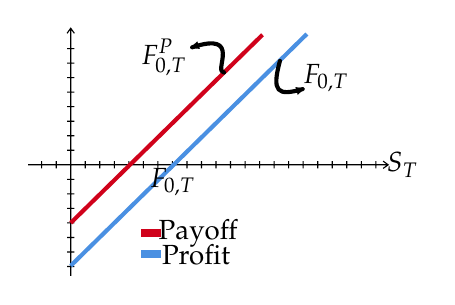
\begin{tikzpicture}[x=0.75pt,y=0.75pt,yscale=-0.35,xscale=0.35]
%uncomment if require: \path (0,363); %set diagram left start at 0, and has height of 363

%Shape: Axis 2D [id:dp37047505143526605] 
\draw  (14,196) -- (509.5,196)(72.5,8) -- (72.5,349) (502.5,191) -- (509.5,196) -- (502.5,201) (67.5,15) -- (72.5,8) -- (77.5,15) (92.5,191) -- (92.5,201)(112.5,191) -- (112.5,201)(132.5,191) -- (132.5,201)(152.5,191) -- (152.5,201)(172.5,191) -- (172.5,201)(192.5,191) -- (192.5,201)(212.5,191) -- (212.5,201)(232.5,191) -- (232.5,201)(252.5,191) -- (252.5,201)(272.5,191) -- (272.5,201)(292.5,191) -- (292.5,201)(312.5,191) -- (312.5,201)(332.5,191) -- (332.5,201)(352.5,191) -- (352.5,201)(372.5,191) -- (372.5,201)(392.5,191) -- (392.5,201)(412.5,191) -- (412.5,201)(432.5,191) -- (432.5,201)(452.5,191) -- (452.5,201)(472.5,191) -- (472.5,201)(492.5,191) -- (492.5,201)(52.5,191) -- (52.5,201)(32.5,191) -- (32.5,201)(67.5,176) -- (77.5,176)(67.5,156) -- (77.5,156)(67.5,136) -- (77.5,136)(67.5,116) -- (77.5,116)(67.5,96) -- (77.5,96)(67.5,76) -- (77.5,76)(67.5,56) -- (77.5,56)(67.5,36) -- (77.5,36)(67.5,216) -- (77.5,216)(67.5,236) -- (77.5,236)(67.5,256) -- (77.5,256)(67.5,276) -- (77.5,276)(67.5,296) -- (77.5,296)(67.5,316) -- (77.5,316)(67.5,336) -- (77.5,336) ;
\draw   ;
%Straight Lines [id:da30565410694888984] 
\draw [color={rgb, 255:red, 208; green, 2; blue, 27 }  ,draw opacity=1 ][line width=1.5]    (72.5,276) -- (336.5,17) ;


%Straight Lines [id:da2716512101716435] 
\draw [color={rgb, 255:red, 74; green, 144; blue, 226 }  ,draw opacity=1 ][line width=1.5]    (72.5,335) -- (397.5,16) ;


%Curve Lines [id:da4305252903013169] 
\draw [color={rgb, 255:red, 0; green, 0; blue, 0 }  ][line width=1.5] [line join = round][line cap = round]   (360.5,53) .. controls (348.8,95.9) and (357.06,101.73) .. (391.78,91.79) ;
\draw [shift={(394.5,91)}, rotate = 523.44] [fill={rgb, 255:red, 0; green, 0; blue, 0 }  ][line width=1.5] [line join = round][line cap = round] [draw opacity=0] (11.61,-5.58) -- (0,0) -- (11.61,5.58) -- cycle    ;

%Curve Lines [id:da29606513394571055] 
\draw [color={rgb, 255:red, 0; green, 0; blue, 0 }  ][line width=1.5] [line join = round][line cap = round]   (283.5,69) .. controls (267.71,69) and (309.65,11.17) .. (239.66,34.28) ;
\draw [shift={(237.5,35)}, rotate = 341.1] [fill={rgb, 255:red, 0; green, 0; blue, 0 }  ][line width=1.5] [line join = round][line cap = round] [draw opacity=0] (11.61,-5.58) -- (0,0) -- (11.61,5.58) -- cycle    ;

%Straight Lines [id:da27180621762709967] 
\draw [color={rgb, 255:red, 208; green, 2; blue, 27 }  ,draw opacity=1 ][line width=3]    (169.5,290) -- (196.5,290) ;


%Straight Lines [id:da47840375462275264] 
\draw [color={rgb, 255:red, 74; green, 144; blue, 226 }  ,draw opacity=1 ][line width=3]    (169.5,319) -- (196.5,319) ;




% Text Node
\draw (529,196) node  [align=left] {$\displaystyle S_{T}$};
% Text Node
\draw (424,77) node  [align=left] {$\displaystyle F_{0,T}$};
% Text Node
\draw (201,48) node  [align=left] {$\displaystyle F^{P}_{0,T}$};
% Text Node
\draw (213,220) node   {$F_{0,T}$};
% Text Node
\draw (248,291) node  [align=left] {Payoff};
% Text Node
\draw (245,320) node  [align=left] {Profit};


\end{tikzpicture}


\end{description}
\paragraph{Achat ferme et emprunt} On utilise parfois la lettre $S$ pour désigner dans stratégie l'action de faire un achat ferme (i.e. acheter et se faire livrer le sous-jacent à $t=0$) et $B$ pour désigner un dépôt/emprunt (qu'on exprime comme une obligation zéro-coupon).


\subsection*{$Call(K,T)$}
Contrat qui \textit{permet} au détenteur de se procurer $S$ au prix $K$ à l'échéance $T$. \textbf{position longue dans le sous-jacent}
\[Premium = C(K,T) \]
\[Payoff =
\begin{cases}
0				& , S_T \leq K \\
S_T - K		& , S_T > K \\
\end{cases}
\]


\tikzset{every picture/.style={line width=0.75pt}} %set default line width to 0.75pt        

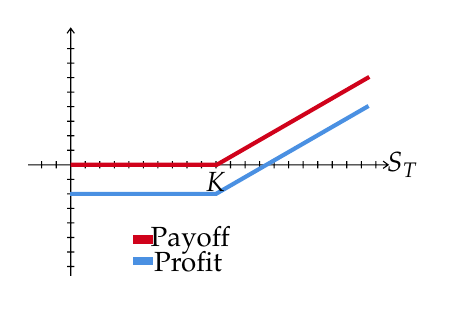
\begin{tikzpicture}[x=0.75pt,y=0.75pt,yscale=-0.35,xscale=0.35]
%uncomment if require: \path (0,363); %set diagram left start at 0, and has height of 363

%Shape: Axis 2D [id:dp5463169858257906] 
\draw  (14,196) -- (509.5,196)(72.5,8) -- (72.5,349) (502.5,191) -- (509.5,196) -- (502.5,201) (67.5,15) -- (72.5,8) -- (77.5,15) (92.5,191) -- (92.5,201)(112.5,191) -- (112.5,201)(132.5,191) -- (132.5,201)(152.5,191) -- (152.5,201)(172.5,191) -- (172.5,201)(192.5,191) -- (192.5,201)(212.5,191) -- (212.5,201)(232.5,191) -- (232.5,201)(252.5,191) -- (252.5,201)(272.5,191) -- (272.5,201)(292.5,191) -- (292.5,201)(312.5,191) -- (312.5,201)(332.5,191) -- (332.5,201)(352.5,191) -- (352.5,201)(372.5,191) -- (372.5,201)(392.5,191) -- (392.5,201)(412.5,191) -- (412.5,201)(432.5,191) -- (432.5,201)(452.5,191) -- (452.5,201)(472.5,191) -- (472.5,201)(492.5,191) -- (492.5,201)(52.5,191) -- (52.5,201)(32.5,191) -- (32.5,201)(67.5,176) -- (77.5,176)(67.5,156) -- (77.5,156)(67.5,136) -- (77.5,136)(67.5,116) -- (77.5,116)(67.5,96) -- (77.5,96)(67.5,76) -- (77.5,76)(67.5,56) -- (77.5,56)(67.5,36) -- (77.5,36)(67.5,216) -- (77.5,216)(67.5,236) -- (77.5,236)(67.5,256) -- (77.5,256)(67.5,276) -- (77.5,276)(67.5,296) -- (77.5,296)(67.5,316) -- (77.5,316)(67.5,336) -- (77.5,336) ;
\draw   ;
%Straight Lines [id:da7976785321827353] 
\draw [color={rgb, 255:red, 208; green, 2; blue, 27 }  ,draw opacity=1 ][line width=1.5]    (72.5,196) -- (273.5,196) -- (483.5,75) ;


%Straight Lines [id:da6660630721177446] 
\draw [color={rgb, 255:red, 74; green, 144; blue, 226 }  ,draw opacity=1 ][line width=1.5]    (71.5,236) -- (272.5,236) -- (482.5,115) ;


%Straight Lines [id:da6103186606436649] 
\draw [color={rgb, 255:red, 208; green, 2; blue, 27 }  ,draw opacity=1 ][line width=3]    (158.5,299) -- (185.5,299) ;


%Straight Lines [id:da7610065512800028] 
\draw [color={rgb, 255:red, 74; green, 144; blue, 226 }  ,draw opacity=1 ][line width=3]    (158.5,328) -- (185.5,328) ;




% Text Node
\draw (529,196) node  [align=left] {$\displaystyle S_{T}$};
% Text Node
\draw (272,220) node   {$K$};
% Text Node
\draw (237,300) node  [align=left] {Payoff};
% Text Node
\draw (234,329) node  [align=left] {Profit};


\end{tikzpicture}




\subsection*{$Put(K,T)$}
Contrat qui \textit{permet} au détenteur de vendre $S$ au prix $K$ à l'échéance $T$. \textbf{position courte dans le sous-jacent}
\[Premium = P(K,T)\]
\[Payoff =
\begin{cases}
K - S_T			& , S_T \leq K \\
0					& , S_T > K \\
\end{cases}
\]


\tikzset{every picture/.style={line width=0.75pt}} %set default line width to 0.75pt        

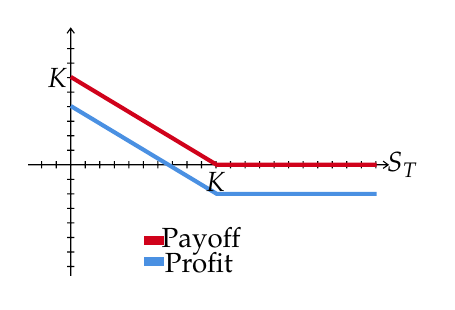
\begin{tikzpicture}[x=0.75pt,y=0.75pt,yscale=-0.35,xscale=0.35]
%uncomment if require: \path (0,363); %set diagram left start at 0, and has height of 363

%Shape: Axis 2D [id:dp32679631247578145] 
\draw  (14,196) -- (509.5,196)(72.5,8) -- (72.5,349) (502.5,191) -- (509.5,196) -- (502.5,201) (67.5,15) -- (72.5,8) -- (77.5,15) (92.5,191) -- (92.5,201)(112.5,191) -- (112.5,201)(132.5,191) -- (132.5,201)(152.5,191) -- (152.5,201)(172.5,191) -- (172.5,201)(192.5,191) -- (192.5,201)(212.5,191) -- (212.5,201)(232.5,191) -- (232.5,201)(252.5,191) -- (252.5,201)(272.5,191) -- (272.5,201)(292.5,191) -- (292.5,201)(312.5,191) -- (312.5,201)(332.5,191) -- (332.5,201)(352.5,191) -- (352.5,201)(372.5,191) -- (372.5,201)(392.5,191) -- (392.5,201)(412.5,191) -- (412.5,201)(432.5,191) -- (432.5,201)(452.5,191) -- (452.5,201)(472.5,191) -- (472.5,201)(492.5,191) -- (492.5,201)(52.5,191) -- (52.5,201)(32.5,191) -- (32.5,201)(67.5,176) -- (77.5,176)(67.5,156) -- (77.5,156)(67.5,136) -- (77.5,136)(67.5,116) -- (77.5,116)(67.5,96) -- (77.5,96)(67.5,76) -- (77.5,76)(67.5,56) -- (77.5,56)(67.5,36) -- (77.5,36)(67.5,216) -- (77.5,216)(67.5,236) -- (77.5,236)(67.5,256) -- (77.5,256)(67.5,276) -- (77.5,276)(67.5,296) -- (77.5,296)(67.5,316) -- (77.5,316)(67.5,336) -- (77.5,336) ;
\draw   ;
%Straight Lines [id:da9604161173645711] 
\draw [color={rgb, 255:red, 208; green, 2; blue, 27 }  ,draw opacity=1 ][line width=1.5]    (72.5,75) -- (273.5,196) -- (493.5,196) ;


%Straight Lines [id:da15996055282562605] 
\draw [color={rgb, 255:red, 208; green, 2; blue, 27 }  ,draw opacity=1 ][line width=3]    (173.5,300) -- (200.5,300) ;


%Straight Lines [id:da4258515905760497] 
\draw [color={rgb, 255:red, 74; green, 144; blue, 226 }  ,draw opacity=1 ][line width=3]    (173.5,329) -- (200.5,329) ;



%Straight Lines [id:da051590301396964966] 
\draw [color={rgb, 255:red, 74; green, 144; blue, 226 }  ,draw opacity=1 ][line width=1.5]    (72.5,115) -- (273.5,236) -- (493.5,236) ;



% Text Node
\draw (529,196) node  [align=left] {$\displaystyle S_{T}$};
% Text Node
\draw (252,301) node  [align=left] {Payoff};
% Text Node
\draw (249,330) node  [align=left] {Profit};
% Text Node
\draw (272,220) node   {$K$};
% Text Node
\draw (54,76) node   {$K$};


\end{tikzpicture}



\subsection*{Forward synthétique}
On peut créer un Forward synthétique 2 de façon (en combinant d'autres transactions) :
\[Forward = Stock - Bond \]
\[Forward = Call(K,T) - Put(K,T) \]
Ces deux égalités définissent la \emph{Put-Call Parity} vu un peu plus loin.


\section{Stratégie de couverture}
\subsection*{Floor}
On achète $S$ en se protégant contre une baisse trop importante du sous-jacent (\textbf{position longue})
\[Floor = Stock + Put(K,T)\]
\[Premium = S_0 + P(K,T) > 0\]
\[Payoff =
\begin{cases}
K					& , S_T \leq K \\
S_T				& , S_T > K \\
\end{cases}
\]


\tikzset{every picture/.style={line width=0.75pt}} %set default line width to 0.75pt        

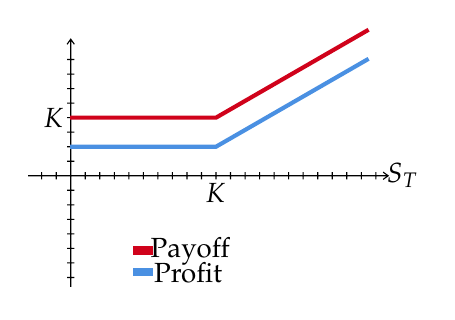
\begin{tikzpicture}[x=0.75pt,y=0.75pt,yscale=-0.35,xscale=0.35]
%uncomment if require: \path (0,363); %set diagram left start at 0, and has height of 363

%Shape: Axis 2D [id:dp5284616222676404] 
\draw  (14,196) -- (509.5,196)(72.5,8) -- (72.5,349) (502.5,191) -- (509.5,196) -- (502.5,201) (67.5,15) -- (72.5,8) -- (77.5,15) (92.5,191) -- (92.5,201)(112.5,191) -- (112.5,201)(132.5,191) -- (132.5,201)(152.5,191) -- (152.5,201)(172.5,191) -- (172.5,201)(192.5,191) -- (192.5,201)(212.5,191) -- (212.5,201)(232.5,191) -- (232.5,201)(252.5,191) -- (252.5,201)(272.5,191) -- (272.5,201)(292.5,191) -- (292.5,201)(312.5,191) -- (312.5,201)(332.5,191) -- (332.5,201)(352.5,191) -- (352.5,201)(372.5,191) -- (372.5,201)(392.5,191) -- (392.5,201)(412.5,191) -- (412.5,201)(432.5,191) -- (432.5,201)(452.5,191) -- (452.5,201)(472.5,191) -- (472.5,201)(492.5,191) -- (492.5,201)(52.5,191) -- (52.5,201)(32.5,191) -- (32.5,201)(67.5,176) -- (77.5,176)(67.5,156) -- (77.5,156)(67.5,136) -- (77.5,136)(67.5,116) -- (77.5,116)(67.5,96) -- (77.5,96)(67.5,76) -- (77.5,76)(67.5,56) -- (77.5,56)(67.5,36) -- (77.5,36)(67.5,216) -- (77.5,216)(67.5,236) -- (77.5,236)(67.5,256) -- (77.5,256)(67.5,276) -- (77.5,276)(67.5,296) -- (77.5,296)(67.5,316) -- (77.5,316)(67.5,336) -- (77.5,336) ;
\draw   ;
%Straight Lines [id:da07170428809155915] 
\draw [color={rgb, 255:red, 208; green, 2; blue, 27 }  ,draw opacity=1 ][line width=1.5]    (71.5,116) -- (272.5,116) -- (482.5,-5) ;


%Straight Lines [id:da9437345853796594] 
\draw [color={rgb, 255:red, 74; green, 144; blue, 226 }  ,draw opacity=1 ][line width=1.5]    (71.5,156) -- (272.5,156) -- (482.5,35) ;


%Straight Lines [id:da10527715337594734] 
\draw [color={rgb, 255:red, 208; green, 2; blue, 27 }  ,draw opacity=1 ][line width=3]    (158.5,299) -- (185.5,299) ;


%Straight Lines [id:da20667043631469095] 
\draw [color={rgb, 255:red, 74; green, 144; blue, 226 }  ,draw opacity=1 ][line width=3]    (158.5,328) -- (185.5,328) ;




% Text Node
\draw (529,196) node  [align=left] {$\displaystyle S_{T}$};
% Text Node
\draw (272,220) node   {$K$};
% Text Node
\draw (237,300) node  [align=left] {Payoff};
% Text Node
\draw (234,329) node  [align=left] {Profit};
% Text Node
\draw (49,117) node   {$K$};


\end{tikzpicture}



\subsection*{Cap}
On vend à découvert $S$ en se protégant contre une hausse trop importante du sous-jacent (car il faudra éventuellement le racheter!). \textbf{Position courte}.
\[Cap = Call(K,T) - Stock\]
\[Premium = C(K,T) - S_0 < 0\]
\[Payoff
\begin{cases}
- S_T 			& , S_T \leq K \\
- K				& , S_T > K \\
\end{cases}
\]


\tikzset{every picture/.style={line width=0.75pt}} %set default line width to 0.75pt        

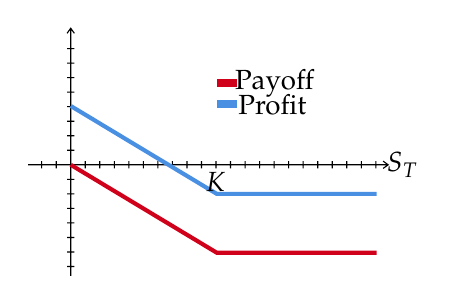
\begin{tikzpicture}[x=0.75pt,y=0.75pt,yscale=-0.35,xscale=0.35]
%uncomment if require: \path (0,363); %set diagram left start at 0, and has height of 363

%Shape: Axis 2D [id:dp037268718196239004] 
\draw  (14,196) -- (509.5,196)(72.5,8) -- (72.5,349) (502.5,191) -- (509.5,196) -- (502.5,201) (67.5,15) -- (72.5,8) -- (77.5,15) (92.5,191) -- (92.5,201)(112.5,191) -- (112.5,201)(132.5,191) -- (132.5,201)(152.5,191) -- (152.5,201)(172.5,191) -- (172.5,201)(192.5,191) -- (192.5,201)(212.5,191) -- (212.5,201)(232.5,191) -- (232.5,201)(252.5,191) -- (252.5,201)(272.5,191) -- (272.5,201)(292.5,191) -- (292.5,201)(312.5,191) -- (312.5,201)(332.5,191) -- (332.5,201)(352.5,191) -- (352.5,201)(372.5,191) -- (372.5,201)(392.5,191) -- (392.5,201)(412.5,191) -- (412.5,201)(432.5,191) -- (432.5,201)(452.5,191) -- (452.5,201)(472.5,191) -- (472.5,201)(492.5,191) -- (492.5,201)(52.5,191) -- (52.5,201)(32.5,191) -- (32.5,201)(67.5,176) -- (77.5,176)(67.5,156) -- (77.5,156)(67.5,136) -- (77.5,136)(67.5,116) -- (77.5,116)(67.5,96) -- (77.5,96)(67.5,76) -- (77.5,76)(67.5,56) -- (77.5,56)(67.5,36) -- (77.5,36)(67.5,216) -- (77.5,216)(67.5,236) -- (77.5,236)(67.5,256) -- (77.5,256)(67.5,276) -- (77.5,276)(67.5,296) -- (77.5,296)(67.5,316) -- (77.5,316)(67.5,336) -- (77.5,336) ;
\draw   ;
%Straight Lines [id:da3847211306528634] 
\draw [color={rgb, 255:red, 208; green, 2; blue, 27 }  ,draw opacity=1 ][line width=1.5]    (72.5,196) -- (273.5,317) -- (493.5,317) ;


%Straight Lines [id:da10620263985508471] 
\draw [color={rgb, 255:red, 208; green, 2; blue, 27 }  ,draw opacity=1 ][line width=3]    (274.5,83) -- (301.5,83) ;


%Straight Lines [id:da0036212401211522804] 
\draw [color={rgb, 255:red, 74; green, 144; blue, 226 }  ,draw opacity=1 ][line width=3]    (274.5,112) -- (301.5,112) ;



%Straight Lines [id:da011019730384494886] 
\draw [color={rgb, 255:red, 74; green, 144; blue, 226 }  ,draw opacity=1 ][line width=1.5]    (72.5,115) -- (273.5,236) -- (493.5,236) ;



% Text Node
\draw (529,196) node  [align=left] {$\displaystyle S_{T}$};
% Text Node
\draw (353,84) node  [align=left] {Payoff};
% Text Node
\draw (350,113) node  [align=left] {Profit};
% Text Node
\draw (272,220) node   {$K$};


\end{tikzpicture}



\subsection*{Bull Spread}
Combinaison de 2 Call (ou 2 Put) pour spéculer sur un marché haussier. Avec $K_1 < K_2$, on a
\paragraph{Avec option d'achat}
\[Bull Spread (Call) = Call(K_1, T) - Call(K_2, T) \]

\[Premium = C(K_1, T) - Call(K_2, T) > 0 \]
\[Payoff =
\begin{cases}
0					& , S_T \leq K_1 \\
S_T - K_1		& , k_1 < S_T \leq K_2 \\
K_2 -K_1		& , S_T > K_2 \\
\end{cases}
\]
\paragraph{Avec option de vente}
\[Bull Spread(Put) = Put(K_1, T) - Put(K_2,T) \]
\[Premium = P(K_1,T) - P(K_2, T) < 0\]
\[Payoff =
\begin{cases}
K_1 - K_2 			& , S_T \leq K_1 \\
K_2 - S_T				& , K_1 < S_T \leq K_2 \\
0							& , S_T > K_2 \\
\end{cases}
\]



\tikzset{every picture/.style={line width=0.75pt}} %set default line width to 0.75pt        

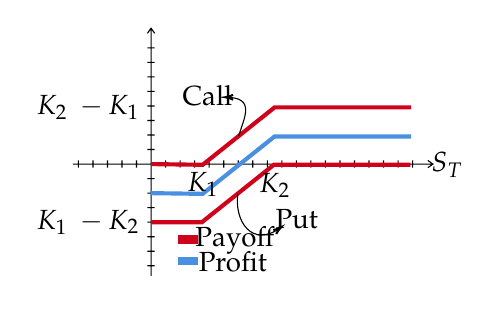
\begin{tikzpicture}[x=0.75pt,y=0.75pt,yscale=-0.35,xscale=0.35]
%uncomment if require: \path (0,363); %set diagram left start at 0, and has height of 363

%Shape: Axis 2D [id:dp28449288707577314] 
\draw  (14,195) -- (509.5,195)(121.5,8) -- (121.5,349) (502.5,190) -- (509.5,195) -- (502.5,200) (116.5,15) -- (121.5,8) -- (126.5,15) (141.5,190) -- (141.5,200)(161.5,190) -- (161.5,200)(181.5,190) -- (181.5,200)(201.5,190) -- (201.5,200)(221.5,190) -- (221.5,200)(241.5,190) -- (241.5,200)(261.5,190) -- (261.5,200)(281.5,190) -- (281.5,200)(301.5,190) -- (301.5,200)(321.5,190) -- (321.5,200)(341.5,190) -- (341.5,200)(361.5,190) -- (361.5,200)(381.5,190) -- (381.5,200)(401.5,190) -- (401.5,200)(421.5,190) -- (421.5,200)(441.5,190) -- (441.5,200)(461.5,190) -- (461.5,200)(481.5,190) -- (481.5,200)(101.5,190) -- (101.5,200)(81.5,190) -- (81.5,200)(61.5,190) -- (61.5,200)(41.5,190) -- (41.5,200)(21.5,190) -- (21.5,200)(116.5,175) -- (126.5,175)(116.5,155) -- (126.5,155)(116.5,135) -- (126.5,135)(116.5,115) -- (126.5,115)(116.5,95) -- (126.5,95)(116.5,75) -- (126.5,75)(116.5,55) -- (126.5,55)(116.5,35) -- (126.5,35)(116.5,215) -- (126.5,215)(116.5,235) -- (126.5,235)(116.5,255) -- (126.5,255)(116.5,275) -- (126.5,275)(116.5,295) -- (126.5,295)(116.5,315) -- (126.5,315)(116.5,335) -- (126.5,335) ;
\draw   ;
%Straight Lines [id:da9209384368986784] 
\draw [color={rgb, 255:red, 208; green, 2; blue, 27 }  ,draw opacity=1 ][line width=1.5]    (121.5,195) -- (192.5,196) -- (291.5,117) -- (479.5,117) ;


%Straight Lines [id:da37977537439547226] 
\draw [color={rgb, 255:red, 208; green, 2; blue, 27 }  ,draw opacity=1 ][line width=3]    (158.5,299) -- (185.5,299) ;


%Straight Lines [id:da9460733927110921] 
\draw [color={rgb, 255:red, 74; green, 144; blue, 226 }  ,draw opacity=1 ][line width=3]    (158.5,328) -- (185.5,328) ;



%Straight Lines [id:da9014316388237789] 
\draw [color={rgb, 255:red, 74; green, 144; blue, 226 }  ,draw opacity=1 ][line width=1.5]    (120.5,235) -- (192.5,236) -- (291.5,157) -- (479.5,157) ;


%Straight Lines [id:da22160788848594903] 
\draw [color={rgb, 255:red, 208; green, 2; blue, 27 }  ,draw opacity=1 ][line width=1.5]    (121.5,275) -- (191.5,275) -- (290.5,196) -- (478.5,196) ;


%Curve Lines [id:da09447744102237843] 
\draw    (241,235.5) .. controls (235.56,272.63) and (260,311.22) .. (299.3,282.88) ;
\draw [shift={(300.5,282)}, rotate = 503.13] [color={rgb, 255:red, 0; green, 0; blue, 0 }  ][line width=0.75]    (10.93,-3.29) .. controls (6.95,-1.4) and (3.31,-0.3) .. (0,0) .. controls (3.31,0.3) and (6.95,1.4) .. (10.93,3.29)   ;

%Curve Lines [id:da08283708021002456] 
\draw    (242,156.5) .. controls (250.37,129.41) and (265.05,103.78) .. (225.35,103.02) ;
\draw [shift={(223.5,103)}, rotate = 360] [color={rgb, 255:red, 0; green, 0; blue, 0 }  ][line width=0.75]    (10.93,-3.29) .. controls (6.95,-1.4) and (3.31,-0.3) .. (0,0) .. controls (3.31,0.3) and (6.95,1.4) .. (10.93,3.29)   ;


% Text Node
\draw (529,196) node  [align=left] {$\displaystyle S_{T}$};
% Text Node
\draw (193,223) node   {$K_{1}$};
% Text Node
\draw (237,300) node  [align=left] {Payoff};
% Text Node
\draw (234,329) node  [align=left] {Profit};
% Text Node
\draw (35,117) node   {$K_{2} \ -K_{1}$};
% Text Node
\draw (292,224) node   {$K_{2}$};
% Text Node
\draw (322,271) node  [align=left] {Put};
% Text Node
\draw (199,101) node  [align=left] {Call};
% Text Node
\draw (35,275) node   {$K_{1} \ -K_{2}$};


\end{tikzpicture}




\subsection*{Bear Spread}
Combinaison de 2 Call ou 2 Put pour spéculer sur un marché baissier.
\paragraph{Avec option d'achat}
\begin{align*}
Bear(Call) & =  - Bull(Call) \\
& = Call(K_2, T) - Call(K_1, T) \\
Premium		& = 	 C(K_2,T) - C(K_1,T) < 0 \\
Profit	& =
\begin{cases}
0					& , S_T \leq K_1 \\
K_1 - S_T 	& , K_1 < S_T \leq K_2 \\
-(K_2 - K_1)& , S_T > K_2 \\
\end{cases}
\end{align*}

\paragraph{Avec option de vente}
\begin{align*}
Bear(Put) 				& =  - Bull(Put) \\
								& = Put(K_2, T) - Put(K_1, T) \\
Premium					& = 	 P(K_2,T) - P(K_1,T) > 0 \\
Profit						& =
\begin{cases}
K_2 - K_1					& , S_T \leq K_1 \\
K_2 - S_T 				& , K_1 < S_T \leq K_2 \\
0								& , S_T > K_2 \\
\end{cases}
\end{align*}


\tikzset{every picture/.style={line width=0.75pt}} %set default line width to 0.75pt        

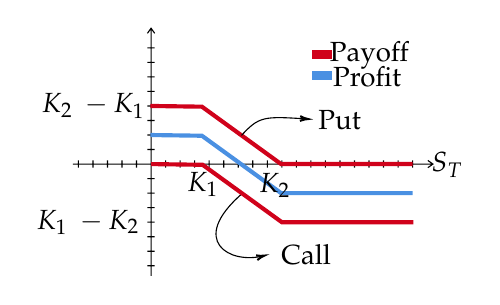
\begin{tikzpicture}[x=0.75pt,y=0.75pt,yscale=-0.35,xscale=0.35]
%uncomment if require: \path (0,363); %set diagram left start at 0, and has height of 363

%Shape: Axis 2D [id:dp5006858190484493] 
\draw  (14,195) -- (509.5,195)(121.5,8) -- (121.5,349) (502.5,190) -- (509.5,195) -- (502.5,200) (116.5,15) -- (121.5,8) -- (126.5,15) (141.5,190) -- (141.5,200)(161.5,190) -- (161.5,200)(181.5,190) -- (181.5,200)(201.5,190) -- (201.5,200)(221.5,190) -- (221.5,200)(241.5,190) -- (241.5,200)(261.5,190) -- (261.5,200)(281.5,190) -- (281.5,200)(301.5,190) -- (301.5,200)(321.5,190) -- (321.5,200)(341.5,190) -- (341.5,200)(361.5,190) -- (361.5,200)(381.5,190) -- (381.5,200)(401.5,190) -- (401.5,200)(421.5,190) -- (421.5,200)(441.5,190) -- (441.5,200)(461.5,190) -- (461.5,200)(481.5,190) -- (481.5,200)(101.5,190) -- (101.5,200)(81.5,190) -- (81.5,200)(61.5,190) -- (61.5,200)(41.5,190) -- (41.5,200)(21.5,190) -- (21.5,200)(116.5,175) -- (126.5,175)(116.5,155) -- (126.5,155)(116.5,135) -- (126.5,135)(116.5,115) -- (126.5,115)(116.5,95) -- (126.5,95)(116.5,75) -- (126.5,75)(116.5,55) -- (126.5,55)(116.5,35) -- (126.5,35)(116.5,215) -- (126.5,215)(116.5,235) -- (126.5,235)(116.5,255) -- (126.5,255)(116.5,275) -- (126.5,275)(116.5,295) -- (126.5,295)(116.5,315) -- (126.5,315)(116.5,335) -- (126.5,335) ;
\draw   ;
%Straight Lines [id:da13258465142858888] 
\draw [color={rgb, 255:red, 208; green, 2; blue, 27 }  ,draw opacity=1 ][line width=1.5]    (120.5,115) -- (191.5,116) -- (300.5,195) -- (481.5,195) ;


%Straight Lines [id:da7932939446362234] 
\draw [color={rgb, 255:red, 208; green, 2; blue, 27 }  ,draw opacity=1 ][line width=3]    (343.5,44) -- (370.5,44) ;


%Straight Lines [id:da14367852228745004] 
\draw [color={rgb, 255:red, 74; green, 144; blue, 226 }  ,draw opacity=1 ][line width=3]    (343.5,73) -- (370.5,73) ;



%Curve Lines [id:da6986177249173428] 
\draw    (246,155.5) .. controls (270.26,129.26) and (276.38,129) .. (335.69,132.88) ;
\draw [shift={(337.5,133)}, rotate = 183.75] [color={rgb, 255:red, 0; green, 0; blue, 0 }  ][line width=0.75]    (10.93,-3.29) .. controls (6.95,-1.4) and (3.31,-0.3) .. (0,0) .. controls (3.31,0.3) and (6.95,1.4) .. (10.93,3.29)   ;

%Curve Lines [id:da16730216097312656] 
\draw    (247,235.5) .. controls (172.25,300.35) and (229.33,333.34) .. (276.09,321.38) ;
\draw [shift={(277.5,321)}, rotate = 524.54] [color={rgb, 255:red, 0; green, 0; blue, 0 }  ][line width=0.75]    (10.93,-3.29) .. controls (6.95,-1.4) and (3.31,-0.3) .. (0,0) .. controls (3.31,0.3) and (6.95,1.4) .. (10.93,3.29)   ;

%Straight Lines [id:da38075245439918526] 
\draw [color={rgb, 255:red, 74; green, 144; blue, 226 }  ,draw opacity=1 ][line width=1.5]    (120.5,155) -- (191.5,156) -- (300.5,235) -- (481.5,235) ;


%Straight Lines [id:da001223510828637031] 
\draw [color={rgb, 255:red, 208; green, 2; blue, 27 }  ,draw opacity=1 ][line width=1.5]    (121.5,195) -- (192.5,196) -- (301.5,275) -- (482.5,275) ;



% Text Node
\draw (529,196) node  [align=left] {$\displaystyle S_{T}$};
% Text Node
\draw (193,223) node   {$K_{1}$};
% Text Node
\draw (422,45) node  [align=left] {Payoff};
% Text Node
\draw (419,74) node  [align=left] {Profit};
% Text Node
\draw (42,115) node   {$K_{2} \ -K_{1}$};
% Text Node
\draw (292,224) node   {$K_{2}$};
% Text Node
\draw (381,134) node  [align=left] {Put};
% Text Node
\draw (335,320) node  [align=left] {Call};
% Text Node
\draw (35,275) node   {$K_{1} \ -K_{2}$};


\end{tikzpicture}



\subsection*{Ratio Spread}
Cette stratégie est une combinaison un peu sur mesure (on ne peut pas nécessairement dire si elle est longue ou courte). On achète $n$ options d'achat à un prix d'exercice $K_1$ et on en vend $m$ à un prix d'exercice $K_2$.\footnote{On peut faire cette stratégie avec des options de vente aussi.}
\begin{align*}
Ratio Spread 		& 	= n Call(K_1, T) - m Call(K_2, T) \\
Premium				& = n C(K_1, T) - m C(K_2,T) \\
Payoff					& = ...
\end{align*}

\subsection*{Box Spread}
Cette stratégie réplique l'achat d'une obligation zéro-coupon, en impliquant 2 option d'achat et 2 options de vente.
\begin{align*}
Box Spread			& = Bull(Call) + Bear(Put) \\
& = Call(K_1, T) - Call(K_2, T)  \\
& + Put(K_2, T) - Put(K_1, T) \\
Premium				& = C(K_1, T) - C(K_2, T) \\
							&  + P(K_2, T) - P(K_1,T) >  0 \\
Payoff					& = K_2 - K_1  \ , \forall S_T \\
\end{align*}


\tikzset{every picture/.style={line width=0.75pt}} %set default line width to 0.75pt        

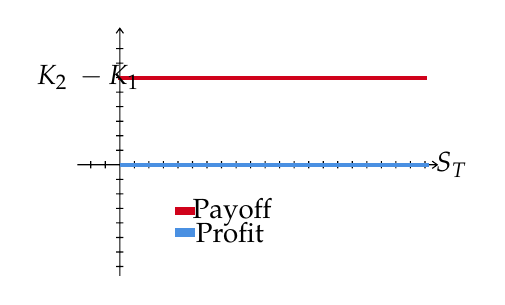
\begin{tikzpicture}[x=0.75pt,y=0.75pt,yscale=-0.35,xscale=0.35]
%uncomment if require: \path (0,363); %set diagram left start at 0, and has height of 363

%Shape: Axis 2D [id:dp6247716683220562] 
\draw  (14,196) -- (509.5,196)(72.5,8) -- (72.5,349) (502.5,191) -- (509.5,196) -- (502.5,201) (67.5,15) -- (72.5,8) -- (77.5,15) (92.5,191) -- (92.5,201)(112.5,191) -- (112.5,201)(132.5,191) -- (132.5,201)(152.5,191) -- (152.5,201)(172.5,191) -- (172.5,201)(192.5,191) -- (192.5,201)(212.5,191) -- (212.5,201)(232.5,191) -- (232.5,201)(252.5,191) -- (252.5,201)(272.5,191) -- (272.5,201)(292.5,191) -- (292.5,201)(312.5,191) -- (312.5,201)(332.5,191) -- (332.5,201)(352.5,191) -- (352.5,201)(372.5,191) -- (372.5,201)(392.5,191) -- (392.5,201)(412.5,191) -- (412.5,201)(432.5,191) -- (432.5,201)(452.5,191) -- (452.5,201)(472.5,191) -- (472.5,201)(492.5,191) -- (492.5,201)(52.5,191) -- (52.5,201)(32.5,191) -- (32.5,201)(67.5,176) -- (77.5,176)(67.5,156) -- (77.5,156)(67.5,136) -- (77.5,136)(67.5,116) -- (77.5,116)(67.5,96) -- (77.5,96)(67.5,76) -- (77.5,76)(67.5,56) -- (77.5,56)(67.5,36) -- (77.5,36)(67.5,216) -- (77.5,216)(67.5,236) -- (77.5,236)(67.5,256) -- (77.5,256)(67.5,276) -- (77.5,276)(67.5,296) -- (77.5,296)(67.5,316) -- (77.5,316)(67.5,336) -- (77.5,336) ;
\draw   ;
%Straight Lines [id:da015831328429750546] 
\draw [color={rgb, 255:red, 208; green, 2; blue, 27 }  ,draw opacity=1 ][line width=3]    (148.5,260) -- (175.5,260) ;


%Straight Lines [id:da9141937301503729] 
\draw [color={rgb, 255:red, 74; green, 144; blue, 226 }  ,draw opacity=1 ][line width=3]    (148.5,289) -- (175.5,289) ;



%Straight Lines [id:da6721376585792007] 
\draw [color={rgb, 255:red, 208; green, 2; blue, 27 }  ,draw opacity=1 ][line width=1.5]    (70.5,76) -- (495.5,76) ;


%Straight Lines [id:da647166999440681] 
\draw [color={rgb, 255:red, 74; green, 144; blue, 226 }  ,draw opacity=1 ][line width=1.5]    (72.5,196) -- (497.5,196) ;



% Text Node
\draw (529,196) node  [align=left] {$\displaystyle S_{T}$};
% Text Node
\draw (227,261) node  [align=left] {Payoff};
% Text Node
\draw (224,290) node  [align=left] {Profit};
% Text Node
\draw (29,76) node   {$K_{2} \ -K_{1}$};


\end{tikzpicture}




\subsection*{Collar}
La prime initiale du Collar peut être soit positive ou négative (dépendant du strike price).
\begin{align*}
Collar				& = Put(K_1, T) - Call(K_2, T) \\
Premium			& = P(K_1, T) - C(K_2,T) \\
Payoff				& =
\begin{cases}
K_1 - S_T			& , S_T \leq K_1 \\
0						& , K_1 < S_T \leq K_2 \\
K_2 - S_T			& , S_T > K_2 \\
\end{cases}
\end{align*}


\tikzset{every picture/.style={line width=0.75pt}} %set default line width to 0.75pt        

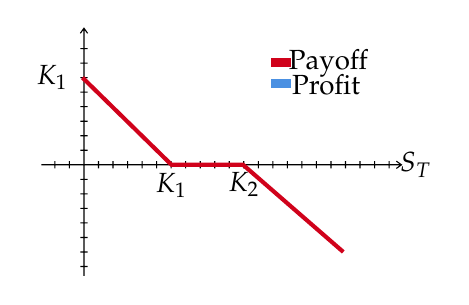
\begin{tikzpicture}[x=0.75pt,y=0.75pt,yscale=-0.35,xscale=0.35]
%uncomment if require: \path (0,363); %set diagram left start at 0, and has height of 363

%Shape: Axis 2D [id:dp6247716683220562] 
\draw  (14,196) -- (509.5,196)(72.5,8) -- (72.5,349) (502.5,191) -- (509.5,196) -- (502.5,201) (67.5,15) -- (72.5,8) -- (77.5,15) (92.5,191) -- (92.5,201)(112.5,191) -- (112.5,201)(132.5,191) -- (132.5,201)(152.5,191) -- (152.5,201)(172.5,191) -- (172.5,201)(192.5,191) -- (192.5,201)(212.5,191) -- (212.5,201)(232.5,191) -- (232.5,201)(252.5,191) -- (252.5,201)(272.5,191) -- (272.5,201)(292.5,191) -- (292.5,201)(312.5,191) -- (312.5,201)(332.5,191) -- (332.5,201)(352.5,191) -- (352.5,201)(372.5,191) -- (372.5,201)(392.5,191) -- (392.5,201)(412.5,191) -- (412.5,201)(432.5,191) -- (432.5,201)(452.5,191) -- (452.5,201)(472.5,191) -- (472.5,201)(492.5,191) -- (492.5,201)(52.5,191) -- (52.5,201)(32.5,191) -- (32.5,201)(67.5,176) -- (77.5,176)(67.5,156) -- (77.5,156)(67.5,136) -- (77.5,136)(67.5,116) -- (77.5,116)(67.5,96) -- (77.5,96)(67.5,76) -- (77.5,76)(67.5,56) -- (77.5,56)(67.5,36) -- (77.5,36)(67.5,216) -- (77.5,216)(67.5,236) -- (77.5,236)(67.5,256) -- (77.5,256)(67.5,276) -- (77.5,276)(67.5,296) -- (77.5,296)(67.5,316) -- (77.5,316)(67.5,336) -- (77.5,336) ;
\draw   ;
%Straight Lines [id:da015831328429750546] 
\draw [color={rgb, 255:red, 208; green, 2; blue, 27 }  ,draw opacity=1 ][line width=3]    (330.5,55) -- (357.5,55) ;


%Straight Lines [id:da9141937301503729] 
\draw [color={rgb, 255:red, 74; green, 144; blue, 226 }  ,draw opacity=1 ][line width=3]    (330.5,84) -- (357.5,84) ;



%Straight Lines [id:da6721376585792007] 
\draw [color={rgb, 255:red, 208; green, 2; blue, 27 }  ,draw opacity=1 ][line width=1.5]    (70.5,76) -- (193,196) -- (291.5,196) -- (429.5,316) ;



% Text Node
\draw (529,196) node  [align=left] {$\displaystyle S_{T}$};
% Text Node
\draw (409,56) node  [align=left] {Payoff};
% Text Node
\draw (406,85) node  [align=left] {Profit};
% Text Node
\draw (29,76) node   {$K_{1}$};
% Text Node
\draw (193,225) node   {$K_{1}$};
% Text Node
\draw (293,223) node   {$K_{2}$};


\end{tikzpicture}




\subsection*{Stock Covered by Collar}
\begin{itemize}
\item On effectue la même stratégie qu'un Collar, en ayant initialement le sous-jacent $S$. \textbf{Position longue dans le sous-jacent}.
\item Cette stratégie reproduit les flux monétaires d'un Bull Spread, alors
\end{itemize}
\begin{align*}
BullSpread				& = Collar + Stock \\
								& = Put(K_1, T) - Call(K_2, T) + Stock \\
Premium					& = P(K_1, T) - C(K_2,T) + S_0 > 0  \\
Payoff						& =
\begin{cases}
K_1 					& , S_T \leq K_1 \\
S_T					& , K_1 < S_T \leq K_2 \\
K_2 					& , S_T > K_2 \\
\end{cases}
\end{align*}


\tikzset{every picture/.style={line width=0.75pt}} %set default line width to 0.75pt        

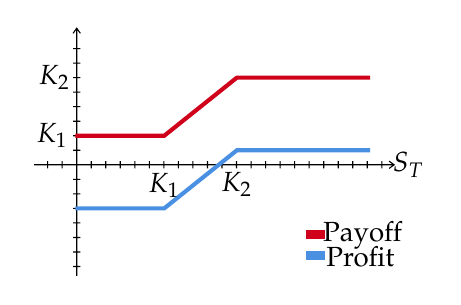
\begin{tikzpicture}[x=0.75pt,y=0.75pt,yscale=-0.35,xscale=0.35]
%uncomment if require: \path (0,363); %set diagram left start at 0, and has height of 363

%Shape: Axis 2D [id:dp20088335764830656] 
\draw  (14,196) -- (509.5,196)(72.5,8) -- (72.5,349) (502.5,191) -- (509.5,196) -- (502.5,201) (67.5,15) -- (72.5,8) -- (77.5,15) (92.5,191) -- (92.5,201)(112.5,191) -- (112.5,201)(132.5,191) -- (132.5,201)(152.5,191) -- (152.5,201)(172.5,191) -- (172.5,201)(192.5,191) -- (192.5,201)(212.5,191) -- (212.5,201)(232.5,191) -- (232.5,201)(252.5,191) -- (252.5,201)(272.5,191) -- (272.5,201)(292.5,191) -- (292.5,201)(312.5,191) -- (312.5,201)(332.5,191) -- (332.5,201)(352.5,191) -- (352.5,201)(372.5,191) -- (372.5,201)(392.5,191) -- (392.5,201)(412.5,191) -- (412.5,201)(432.5,191) -- (432.5,201)(452.5,191) -- (452.5,201)(472.5,191) -- (472.5,201)(492.5,191) -- (492.5,201)(52.5,191) -- (52.5,201)(32.5,191) -- (32.5,201)(67.5,176) -- (77.5,176)(67.5,156) -- (77.5,156)(67.5,136) -- (77.5,136)(67.5,116) -- (77.5,116)(67.5,96) -- (77.5,96)(67.5,76) -- (77.5,76)(67.5,56) -- (77.5,56)(67.5,36) -- (77.5,36)(67.5,216) -- (77.5,216)(67.5,236) -- (77.5,236)(67.5,256) -- (77.5,256)(67.5,276) -- (77.5,276)(67.5,296) -- (77.5,296)(67.5,316) -- (77.5,316)(67.5,336) -- (77.5,336) ;
\draw   ;
%Straight Lines [id:da10536374065219245] 
\draw [color={rgb, 255:red, 208; green, 2; blue, 27 }  ,draw opacity=1 ][line width=3]    (387.5,292) -- (414.5,292) ;


%Straight Lines [id:da016662989001628326] 
\draw [color={rgb, 255:red, 74; green, 144; blue, 226 }  ,draw opacity=1 ][line width=3]    (387.5,321) -- (414.5,321) ;



%Straight Lines [id:da4381336728182633] 
\draw [color={rgb, 255:red, 208; green, 2; blue, 27 }  ,draw opacity=1 ][line width=1.5]    (70.5,156) -- (193,156) -- (293,76) -- (476.5,76) ;


%Straight Lines [id:da9741273233770525] 
\draw [color={rgb, 255:red, 74; green, 144; blue, 226 }  ,draw opacity=1 ][line width=1.5]    (70.5,256) -- (193,256) -- (293,176) -- (476.5,176) ;



% Text Node
\draw (529,196) node  [align=left] {$\displaystyle S_{T}$};
% Text Node
\draw (466,293) node  [align=left] {Payoff};
% Text Node
\draw (463,322) node  [align=left] {Profit};
% Text Node
\draw (39,156) node   {$K_{1}$};
% Text Node
\draw (193,225) node   {$K_{1}$};
% Text Node
\draw (293,223) node   {$K_{2}$};
% Text Node
\draw (42,76) node   {$K_{2}$};


\end{tikzpicture}




\subsection*{Straddle}
Stratégie pour spéculer sur la volatilité du sous-jacent $S$ autour du point $K$.
\begin{align*}
Straddle			& = Put(K,T) + Call(K,T) \\
Premium			& = P(K,T) + C(K,T) > 0 \\
Payoff				& =
\begin{cases}
K - S_T				& , S_T \leq K \\
S_T - K				& , S_T > K \\
\end{cases}
\end{align*}


\tikzset{every picture/.style={line width=0.75pt}} %set default line width to 0.75pt        

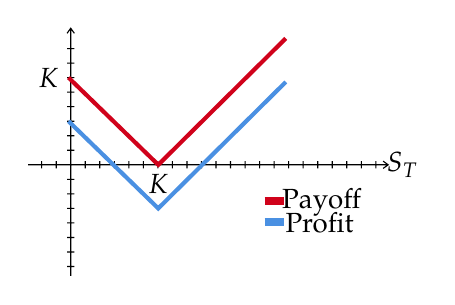
\begin{tikzpicture}[x=0.75pt,y=0.75pt,yscale=-0.35,xscale=0.35]
%uncomment if require: \path (0,363); %set diagram left start at 0, and has height of 363

%Shape: Axis 2D [id:dp04893296182422047] 
\draw  (14,196) -- (509.5,196)(72.5,8) -- (72.5,349) (502.5,191) -- (509.5,196) -- (502.5,201) (67.5,15) -- (72.5,8) -- (77.5,15) (92.5,191) -- (92.5,201)(112.5,191) -- (112.5,201)(132.5,191) -- (132.5,201)(152.5,191) -- (152.5,201)(172.5,191) -- (172.5,201)(192.5,191) -- (192.5,201)(212.5,191) -- (212.5,201)(232.5,191) -- (232.5,201)(252.5,191) -- (252.5,201)(272.5,191) -- (272.5,201)(292.5,191) -- (292.5,201)(312.5,191) -- (312.5,201)(332.5,191) -- (332.5,201)(352.5,191) -- (352.5,201)(372.5,191) -- (372.5,201)(392.5,191) -- (392.5,201)(412.5,191) -- (412.5,201)(432.5,191) -- (432.5,201)(452.5,191) -- (452.5,201)(472.5,191) -- (472.5,201)(492.5,191) -- (492.5,201)(52.5,191) -- (52.5,201)(32.5,191) -- (32.5,201)(67.5,176) -- (77.5,176)(67.5,156) -- (77.5,156)(67.5,136) -- (77.5,136)(67.5,116) -- (77.5,116)(67.5,96) -- (77.5,96)(67.5,76) -- (77.5,76)(67.5,56) -- (77.5,56)(67.5,36) -- (77.5,36)(67.5,216) -- (77.5,216)(67.5,236) -- (77.5,236)(67.5,256) -- (77.5,256)(67.5,276) -- (77.5,276)(67.5,296) -- (77.5,296)(67.5,316) -- (77.5,316)(67.5,336) -- (77.5,336) ;
\draw   ;
%Straight Lines [id:da29326132274692995] 
\draw [color={rgb, 255:red, 208; green, 2; blue, 27 }  ,draw opacity=1 ][line width=3]    (339.5,246) -- (366.5,246) ;


%Straight Lines [id:da0682309073045051] 
\draw [color={rgb, 255:red, 74; green, 144; blue, 226 }  ,draw opacity=1 ][line width=3]    (339.5,275) -- (366.5,275) ;



%Straight Lines [id:da6416016306991924] 
\draw [color={rgb, 255:red, 208; green, 2; blue, 27 }  ,draw opacity=1 ][line width=1.5]    (69.5,76) -- (193,196) -- (368.5,22) ;


%Straight Lines [id:da08174726568750468] 
\draw [color={rgb, 255:red, 74; green, 144; blue, 226 }  ,draw opacity=1 ][line width=1.5]    (69.5,136) -- (193,256) -- (368.5,82) ;



% Text Node
\draw (529,196) node  [align=left] {$\displaystyle S_{T}$};
% Text Node
\draw (418,247) node  [align=left] {Payoff};
% Text Node
\draw (415,276) node  [align=left] {Profit};
% Text Node
\draw (193,223) node   {$K$};
% Text Node
\draw (42,76) node   {$K$};


\end{tikzpicture}



\subsection*{Strangle}
Même genre de stratégie que le strangle, on spécule sur la volatilité du sous-jacent à l'extérieur de l'intervalle $[K_1, K_2]$ :
\begin{align*}
Strangle			& = Put(K_1, T) + Call(K_2, T) \\
Premium			& = P(K_1, T) + C(K_2, T) > 0 \\
Payoff				& =
\begin{cases}
K_1 - S_T			& , S_T \leq K_1 \\
0						& , K_1 < S_T \leq K_2 \\
S_T - K_2 		& , S_T > K_2 \\
\end{cases}
\end{align*}


\tikzset{every picture/.style={line width=0.75pt}} %set default line width to 0.75pt        

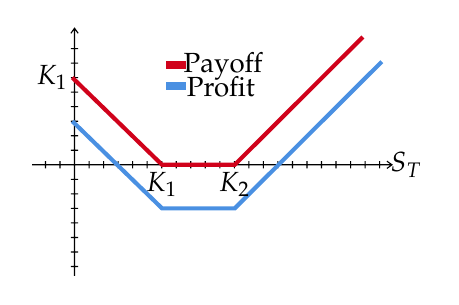
\begin{tikzpicture}[x=0.75pt,y=0.75pt,yscale=-0.35,xscale=0.35]
%uncomment if require: \path (0,363); %set diagram left start at 0, and has height of 363

%Shape: Axis 2D [id:dp20173159090508463] 
\draw  (14,196) -- (509.5,196)(72.5,8) -- (72.5,349) (502.5,191) -- (509.5,196) -- (502.5,201) (67.5,15) -- (72.5,8) -- (77.5,15) (92.5,191) -- (92.5,201)(112.5,191) -- (112.5,201)(132.5,191) -- (132.5,201)(152.5,191) -- (152.5,201)(172.5,191) -- (172.5,201)(192.5,191) -- (192.5,201)(212.5,191) -- (212.5,201)(232.5,191) -- (232.5,201)(252.5,191) -- (252.5,201)(272.5,191) -- (272.5,201)(292.5,191) -- (292.5,201)(312.5,191) -- (312.5,201)(332.5,191) -- (332.5,201)(352.5,191) -- (352.5,201)(372.5,191) -- (372.5,201)(392.5,191) -- (392.5,201)(412.5,191) -- (412.5,201)(432.5,191) -- (432.5,201)(452.5,191) -- (452.5,201)(472.5,191) -- (472.5,201)(492.5,191) -- (492.5,201)(52.5,191) -- (52.5,201)(32.5,191) -- (32.5,201)(67.5,176) -- (77.5,176)(67.5,156) -- (77.5,156)(67.5,136) -- (77.5,136)(67.5,116) -- (77.5,116)(67.5,96) -- (77.5,96)(67.5,76) -- (77.5,76)(67.5,56) -- (77.5,56)(67.5,36) -- (77.5,36)(67.5,216) -- (77.5,216)(67.5,236) -- (77.5,236)(67.5,256) -- (77.5,256)(67.5,276) -- (77.5,276)(67.5,296) -- (77.5,296)(67.5,316) -- (77.5,316)(67.5,336) -- (77.5,336) ;
\draw   ;
%Straight Lines [id:da06729302961101102] 
\draw [color={rgb, 255:red, 208; green, 2; blue, 27 }  ,draw opacity=1 ][line width=3]    (198.5,59) -- (225.5,59) ;


%Straight Lines [id:da7015689476766018] 
\draw [color={rgb, 255:red, 74; green, 144; blue, 226 }  ,draw opacity=1 ][line width=3]    (198.5,88) -- (225.5,88) ;



%Straight Lines [id:da5683323894945758] 
\draw [color={rgb, 255:red, 208; green, 2; blue, 27 }  ,draw opacity=1 ][line width=1.5]    (69.5,76) -- (193,196) -- (293,196) -- (469.5,20) ;


%Straight Lines [id:da06098365181250487] 
\draw [color={rgb, 255:red, 74; green, 144; blue, 226 }  ,draw opacity=1 ][line width=1.5]    (69.5,136) -- (193,256) -- (293,256) -- (495.5,54) ;



% Text Node
\draw (529,196) node  [align=left] {$\displaystyle S_{T}$};
% Text Node
\draw (277,60) node  [align=left] {Payoff};
% Text Node
\draw (274,89) node  [align=left] {Profit};
% Text Node
\draw (193,223) node   {$K_{1}$};
% Text Node
\draw (42,76) node   {$K_1$};
% Text Node
\draw (293,223) node   {$K_{2}$};


\end{tikzpicture}




\subsection*{Butterfly Spread (BFS)}
On combine un Straddle($K_2$) et un Strangle($K_1, K_3$) pour spéculer sur la non-volatilité du sous-jacent autour de $K_2$, mais en limitant nos pertes à $K_1 - K_2$ :
\begin{align*}
Butterfly  & = Strangle - Straddle(K_2) \\
& = Put(K_1, T) - Put(K_2, T) \\
& - Call(K_2, T) + Call(K_3,T) \\
Premium	& = P(K_1, T) - P(K_2, T) \\
& - C(K_2, T) + C(K_3, T) < 0\\
Payoff		& =
\begin{cases}
K_1 - K_2			& , S_T \leq K_1 \\
S_T - K_2			& , K_1 < S_T \leq K_2 \\
K_2 - S_T			& , K_2 < S_T \leq K_3 \\
K_2 - K_3			& , S_T > K_3 \\
\end{cases}
\end{align*}
\paragraph{Note} De façon générale (plusieurs combinaisons sont possibles), on a
\[BFS = Bull(K_1, K_2) + Bear(K_2, K_3) \]


\tikzset{every picture/.style={line width=0.75pt}} %set default line width to 0.75pt        

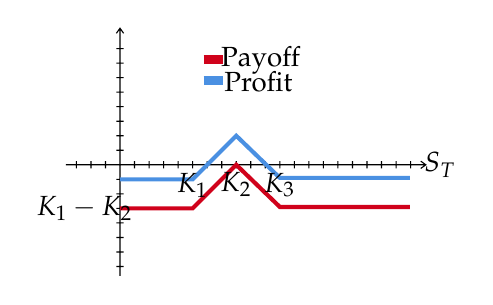
\begin{tikzpicture}[x=0.75pt,y=0.75pt,yscale=-0.35,xscale=0.35]
%uncomment if require: \path (0,363); %set diagram left start at 0, and has height of 363

%Shape: Axis 2D [id:dp516021239542077] 
\draw  (14,196) -- (509.5,196)(88.5,8) -- (88.5,349) (502.5,191) -- (509.5,196) -- (502.5,201) (83.5,15) -- (88.5,8) -- (93.5,15) (108.5,191) -- (108.5,201)(128.5,191) -- (128.5,201)(148.5,191) -- (148.5,201)(168.5,191) -- (168.5,201)(188.5,191) -- (188.5,201)(208.5,191) -- (208.5,201)(228.5,191) -- (228.5,201)(248.5,191) -- (248.5,201)(268.5,191) -- (268.5,201)(288.5,191) -- (288.5,201)(308.5,191) -- (308.5,201)(328.5,191) -- (328.5,201)(348.5,191) -- (348.5,201)(368.5,191) -- (368.5,201)(388.5,191) -- (388.5,201)(408.5,191) -- (408.5,201)(428.5,191) -- (428.5,201)(448.5,191) -- (448.5,201)(468.5,191) -- (468.5,201)(488.5,191) -- (488.5,201)(68.5,191) -- (68.5,201)(48.5,191) -- (48.5,201)(28.5,191) -- (28.5,201)(83.5,176) -- (93.5,176)(83.5,156) -- (93.5,156)(83.5,136) -- (93.5,136)(83.5,116) -- (93.5,116)(83.5,96) -- (93.5,96)(83.5,76) -- (93.5,76)(83.5,56) -- (93.5,56)(83.5,36) -- (93.5,36)(83.5,216) -- (93.5,216)(83.5,236) -- (93.5,236)(83.5,256) -- (93.5,256)(83.5,276) -- (93.5,276)(83.5,296) -- (93.5,296)(83.5,316) -- (93.5,316)(83.5,336) -- (93.5,336) ;
\draw   ;
%Straight Lines [id:da9881769874738698] 
\draw [color={rgb, 255:red, 208; green, 2; blue, 27 }  ,draw opacity=1 ][line width=3]    (203.5,51) -- (230.5,51) ;


%Straight Lines [id:da972554603165243] 
\draw [color={rgb, 255:red, 74; green, 144; blue, 226 }  ,draw opacity=1 ][line width=3]    (203.5,80) -- (230.5,80) ;



%Straight Lines [id:da5214606141485839] 
\draw [color={rgb, 255:red, 208; green, 2; blue, 27 }  ,draw opacity=1 ][line width=1.5]    (88.5,256) -- (188.5,256) -- (248.5,196) -- (308.5,254) -- (487.5,254) ;


%Straight Lines [id:da6207165128721853] 
\draw [color={rgb, 255:red, 74; green, 144; blue, 226 }  ,draw opacity=1 ][line width=1.5]    (88.5,216) -- (188.5,216) -- (248.5,156) -- (308.5,214) -- (487.5,214) ;



% Text Node
\draw (529,196) node  [align=left] {$\displaystyle S_{T}$};
% Text Node
\draw (282,52) node  [align=left] {Payoff};
% Text Node
\draw (279,81) node  [align=left] {Profit};
% Text Node
\draw (188.5,224) node   {$K_{1}$};
% Text Node
\draw (308.5,224) node   {$K_{3}$};
% Text Node
\draw (248.5,223) node   {$K_{2}$};
% Text Node
\draw (40,256) node   {$K_{1} -K_{2}$};


\end{tikzpicture}



\paragraph{Asymetric Butterfly Spread}
\begin{itemize}
\item Comme le Ratio Spread, il est possible de faire une stratégie sur mesure en achetant $n$ Bull Spread et en achetant $m$ Bear Spread en respectant les 3 prix d'exercices $K_1 < K_2 < K_3$.
\item Si on désire avoir un BFS qui a un profit nul pour $S_T < K_1$ et $S_T > K_3$, alors on trouve $n$ et $m$ tel que
\begin{align*}
\frac{n}{m} = \frac{K_3 - K_2}{K_2 - K_1}
\end{align*}
\end{itemize}

% --- Chapitre 5 ---
% J'ai rassemblé une partie de la matière du chap.5 dans le chapitre 9, étant donné qu'on répétait de l'information.
\setcounter{section}{4}
\section{Forwards et Futures}
\subsection*{Forward avec dividendes}
\paragraph{Définition de base}
\[C(K,T) - P(K,T) = S_0 - K(1+r_f)^{T}\]

\paragraph{Action qui verse des dividendes}
\begin{align*}
C(K,T) - P(K,T) 		& = S - \text{PV}(Div) - K(1 + r_f)^{T} \\
& = S_0 e^{-\delta T} - K e^{-rT}
\end{align*}
où $\delta$ est un taux de versement des dividendes continu. \\

De plus, on a
\begin{align*}
F_{0,T} & = F_{0,T}^{P} (1 + r_f)^{T} \\
& = (S_0 - \text{PV}(div))(1+r_f)^{T} \\
& = S_0 - \sum_{i=1}^{T} d_i (1+r_f)^{T-i} \\
& = S_0 e^{(r-\delta)T}
\end{align*}

\paragraph{Forward synthétique avec dividendes}
On suppose le réinvestissement des dividendes.
\begin{align*}
\text{Forward}_{\text{avec div.}} & = e^{-\delta T} Stock - (e^{-\delta T} \cdot S_0) Bond \\
Premium		& =  e^{-\delta T} S_0 - e^{-\delta T} S_0 = 0 \\
Payoff			& = S_T - S_0 e^{(r-\delta) T}
\end{align*}

\paragraph{Cash-and-carry}
Stratégie qui consiste  à créer un Forward synthétique et vendre un Forward (profit nul).


\subsection*{Calcul avec prime de risque et nuance}
\begin{itemize}
\item Certains sous-jacent ont une composante de risque non-négligeable. Or, on ne peut pas dire que $F_{0,T} = \esp{S_T}$. Toutefois,
\[F_{0,T} = \esp{S_T} e^{-(\alpha - r) T}\]
\end{itemize}
où $\alpha$ est la prime de risque 	qu'on enlève pour obtenir le prix du Forward, tel que
\[\alpha = \underbrace{r}_{\text{Taux sans risque}} + \underbrace{(\alpha - r)}_{\text{Prime de risque}}\]

\subsection*{Forward de devise}
\paragraph{Put-Call parity avec les devises}
\begin{description}
\item[DD] Devise locale
\item[DÉ] Device étrangère
\item[$x_0$] Taux de change $\frac{DD}{DÉ}$ actuel ($t=0$)
\item[$r_D$] Taux sans risque \underline{local}
\item[$r_{É}$] Taux sans risque étranger
\end{description}
Le prix Forward prépayé pour une unité de DÉ à $t =0$ (payé en DD) est
\[F_{0,T}^{P}  = x_0 \left(1 + r_{É} \right)^{-T} \]
Et le prix Forward (à $t = T$) pour une unité de DÉ est
\begin{align*}
F_{0,T} & = F_{0,T}^{P} \left(1+r_D \right)^{T} \\
& = x_0 \left(  \frac{1+r_D}{1+r_{É}}   \right)^{T}\\
&  = x_0 e^{(r_D - r_{É})T}
\end{align*}

\paragraph{Forward synthétique de devise}
\begin{itemize}
\item Emprunt de $x_0(1+r_{É})^{-T}$ DD au taux $r_D$
\item Convertir les DD en DÉ
\item Dépôt de $(1+r_{É})^{-T}$ DÉ (au taux $r_{É}$) de 0 à $T$.
\end{itemize}
Le payoff sera $x_t - x_0 \left(  \frac{1+r_D}{1+r_{É}}   \right)^{T}$.


\subsection*{Future}
Essentiellement la même chose qu'un Forward, à quelques différences près :
\begin{itemize}
\item Surveillé et contrôlé par des instances officielles (aucun \textit{Over-the-counter})
\item S'applique sur certains types d'actifs définis seulement ;
\item liquise et efficient
\item nécessite un dépôt initial des 2 parties (le risque de défaut est minimisé)
\item Transaction continues (règlement avec l'intermédiaire de façon quotidienne)
\item Variation extrêmes dans les prix de Future sont limités (possibilité du \textit{circuit Breaker})
\end{itemize}

\paragraph{Fonctionnement}
\begin{enumerate}
\item L'intermédaire demande un dépôt initial (\textit{initial margin}), \textbf{souvent un \% de la valeur notionnelle}.
\item Ce dépôt est accumulé à un taux de rendement $i$ fixé par l'intermédiaire.
\item À chaque période de règlement, on calcule la marge en fonction du prix du Future : \\
$\text{Marge}_T = \text{Marge}_{t} \cdot (1+i)^{T-t} + \text{Variation totale}_{[t,T]}$
\item Si $\text{Marge}_t  < \text{Maintenance margin}$\footnote{Cette marge est souvent exprimée en \% de la marge initiale.}, on doit \textbf{ajouter des fonds à la marge pour revenir à la marge initiale.}
avec $t < T$
\end{enumerate}



% --- Chapitre 9 ---
\setcounter{section}{8}
\section{Put-Call Parity}
\begin{align*}
Call - Put = Stock - Bond
\end{align*}

\subsection*{Put-Call Parity avec devises}
\begin{description}
\item[$Call(x_0, K, T)$ : ] Option d'achat qui permet d'acheter 1 unité de DÉ pour K unité de DD à l'échéance $t = T$.
\item[$Put(x_0, K, T)$ : ] Option de vente qui permet d'acheter 1 unité de DÉ pour K unité de DD à l'échéance $t = T$.
\end{description}
Alors, on peut réécrire l'équation Put-Call Parity :
\begin{align*}
Call(x_0, K,T) - Put(x_0, K, T) = x_0(1+r_{É})^{-T} - K(1+r_D)^{-T}
\end{align*}


\subsection*{Parité généralisée et option d'échange}
\begin{description}
\item[$Call(S_t, Q_t, T - t)$ : ] Option d'achat qui permet d'acheter le sous-jacent $S$ au prix du sous-jacent $Q$ au temps $t = T$.
\item[$Put(S_t, Q_t, T - t)$ : ] Option de vente qui permet de vendre le sous-jacent $S$ au prix du sous-jacent $Q$ au temps $t = T$.
\end{description}
On peut généraliser l'équation Put-Call Parity :
\begin{align*}
C(S_t, Q_t, T - t) - P(S_t, Q_t, T-t) = F_{t,T}^{P}(S) - F_{t,T}^{P}(Q)
\end{align*}

\subsection*{Options sur devise}
\begin{align*}
Call_{DD}(x_0, K, T) & = K \cdot Put_{DD}\left( \frac{1}{x_0}, \frac{1}{K}, T \right) \\
& = K \cdot x_0 \cdot Put_{DÉ} \left( \frac{1}{x_0}, \frac{1}{K}, T \right) \\
\end{align*}


\subsection*{Comparaison de différentes options}
\paragraph{Option américaine vs européenne}
\begin{align*}
C_{amer}(K,T) & \geq C_{euro}(K,T) \\
P_{amer}(K,T) & \geq P_{euro}(K,T) \\
\end{align*}

\paragraph{Option d'achat américaine}
Bien qu'on puisse exercer l'option américaine au moment qu'on veut, il \underline{peut} être optimal d'exercer avant l'échéance seulement si
\begin{align*}
PV(div) > K \left(1 - (1+r_f)^{-(T-t)} \right)
\end{align*}
ou si
\begin{align*}
PV(div) > P(K, T-t) + K \left(1 - (1+r_f)^{-(T-t)} \right)
\end{align*}

\paragraph{Option de vente américaine}
Le moment optimal pour exercer le Put serait tout juste \textbf{après la date ex-dividende}.



\paragraph{Date d'expiration}
Pour $T_1 < T_2$,
\begin{align*}
C(K, T_1) & \leq C(K, T_2) \\
P(K, T_1) & \leq P(K, T_2)
\end{align*}


\paragraph{Prix d'exercice}
Les différentes conditions énumérées ci-bas doivent être respectées :
\begin{tabbing}
\hspace{5cm}\=\kill
 $C(K,T) \geq S_0 - K$ \>  $ P(K,T) \geq K - S_0$ \\
  $C(K_1, T) > C(K_2, T)$ \> $P(K_1, T) < P(K_2, T)$ \\
 $C(K_1, T) - C(K_2, T) \leq K_2 - K_1$ \> $P(K_2, T) - P(K_1, T) \leq K_2 - K_1$ \\
 $\frac{C(K_1, T) - C(K_2, T)}{K_2 - K_1} \geq \frac{C(K_2, T) - C(K_3, T)}{K_3 - K_2}$ \>  $\frac{P(K_2, T) - P(K_1, T)}{K_2 - K_1} \geq \frac{P(K_3, T) - P(K_2, T)}{K_3 - K_2}$ \\
\end{tabbing}
Si le prix d'exercice est \textit{Constant en valeur actualisée}\footnote{i.e. $K_t = K(1+r_f)^{T}$.}, alors, avec $t < T$
\begin{align*}
C(K_t, t) & \leq C(K_T, T) \\
P(K_t, t) & \leq P(K_T, T) \\
\end{align*}

% --- Chapitre 10 ---
\section{Introduction au modèle binomial d'évaluation des options}
\subsection*{Probabilité neutre au risque}
\begin{itemize}
\item $U = uS$ est la valeur supérieure que peut prendre le sous-jacent $S$
\item $D = dS$ est la valeur inférieure que peut prendre le sous-jacent $S$
\item $p$ est la probabilité (Bernouilli) que le sous-jacent prenne la valeur $U$.
\item $\theta_u$ et $\theta_d$ sont les payoff de l'option (Call ou Put) aux branches \emph{up} et \emph{down} respectivement après $h$ périodes.
\item $r$ et $\delta$ sont respectivement la force d'intérêt sans risque et le taux de dividende continu.
\end{itemize}
 Alors, la probabilité \textit{neutre au risque} est
\begin{align*}
p* = \frac{e^{(r-\delta)h} - d}{u-d}
\end{align*}

\subsection*{Portefeuille réplicatif d'une option}
On peut reproduire une option (Call ou Put) avec la stratégie suivante  :
\[C = \Delta S + B\]
où $B$ et $\Delta S$ changent de signe selon si c'est un Call ou un Put. On peut obtenir la prime initiale (\textit{Premium}) et les composantes du portefeuille réplicatif avec
\begin{align*}
\Delta = e^{-\delta h} \left( \frac{\theta_u - \theta_d}{U - D} \right) =   e^{-\delta h} \left( \frac{\theta_u - \theta_d}{S(u -d)} \right)
\end{align*}
\begin{align*}
B = e^{-rh} \left( \frac{U \cdot \theta_d - D \cdot \theta_u}{U - D} \right) = e^{-rh} \left( \frac{u \theta_d - d \theta_u}{u-d} \right)
\end{align*}
où $\theta_u$ et $\theta_d$ sont les \emph{payoff} pour la branche \emph{up} et la branche \emph{down} respectivement.
\begin{align*}
\text{Premium} = \Delta S_0 + B
\end{align*}


\subsection*{Paramètre $u$, $d$ et $\sigma$}
\begin{align*}
	u & = e^{(r-\delta)h + \sigma \sqrt{h}} \\
	d & = e^{(r-\delta)h - \sigma \sqrt{h}} \\
\end{align*}

\subsection*{Rendements composés continûment}
\begin{align*}
	r_{t,t+h} = \ln \left( \frac{S_{t+h}}{S_t} \right)
\end{align*}


\subsection*{Calcul du prix de l'option}
Dans le modèle d'arbre binomial, on peut calculer le prix d'une option $C(K,h)$ comme
\begin{align*}
	C(K,h) = (p^* \theta_u + (1-p^*)\theta_d) e^{-rh}
\end{align*}



On peut trouver la volatilité \underline{annuelle} telle que
\begin{align*}
	\sigma = \frac{\ln \left( u/d \right)}{2 \sqrt{h}}
\end{align*}
Sinon, on peut l'estimer somme la variance non-biaisée des rendements historiques :
\begin{align*}
	\hat{\sigma} = \frac{\sum_{t=1}^{n} (r_{t, t+1} - \bar{r})^2}{(n-1)\sqrt{h}}
\end{align*}
avec $\bar{r} = \frac{1}{n} \sum_{t=1}^n r_t$.

\subsection*{Construction d'un arbre binomial}
\begin{enumerate}
	\item On construit l'arbre de gauche à droite. À chaque noeud, on calcule le prix de l'action et le \emph{payoff} selon le type d'action.
	\item On calcule le prix de l'option et les composantes du portefeuille réplicatif à chaque noeud en fonction des branches $u$ et $d$ de droite à gauche.
	\item Si l'option est de type américaine, il faut vérifier à chaque noeud si il est plus avantageux d'exécuter l'option ou d'attendre (i.e. si le prix de l'option est plus élevé, on attend)
\end{enumerate}


\subsection*{Options sur devise}
Ce sont exactement les même formules, à l'exception qu'on précise le taux sans risque $r_f$ pour le taux sans risque de la devise domestique $r_{DD}$ et le taux de dividende $\delta$ devient le taux sans risque de la domestique étrangère $r_{DÉ}$.




\section{Évaluation des options par la méthode binomiale}


% Début chapitre 12
\section{Formule de Black-Scholes}
\begin{align*}
C(S_0, K, r, \sigma, T, \delta) & = S_0 e^{-\delta T} N(d_1) - K e^{-rT} N(d_2) \\
P(S_0, K, r, \sigma, T, \delta) & = K e^{-rT} N(-d_2) - S_0 e^{-\delta T} N(-d_1)
\end{align*}
avec 
\[d_1 = \frac{\ln \left( \frac{S_0}{K}  \right) + \left( r - \delta + \frac{\sigma^2}{2} \right) }{\sigma \sqrt{T}}  \ \ \  \text{ et } d_2 = d_1 - \sigma \sqrt{T}\]

\subsection*{B-S pour Forward prépayés}
\begin{align*}
C(S, K, r, \sigma, T , \delta) & = F_{0,T}^{P}(S) N(d_1) - F_{0,T}^{P}(K) N(d_2) \\
P(S, K, r, \sigma, T , \delta)  & = F_{0,T}^{P}(K) N(-d_2) - F_{0,T}^{P}(S) N(-d_1)
\end{align*}

\subsection*{B-S pour options avec actions versant des dividendes}

\paragraph{Dividendes discrets proportionnels} Soit $\phi$ un taux de dividende (une proportion de l'action) versé à intervalle régulier. On connaît d'avance le nombre $n$ de dividendes qui seront versés d'ici l'échéance $T$. Alors,
\begin{align*}
C(S, K, r, \sigma, T , \phi) = S(1 - \phi)^{n} N(d_1) - K e^{-rT} N(d_2)
\end{align*}

\paragraph{Dividendes discrets fixes} On suppose que les dividendes $d_t$ sont verrés à des moments connus d'avance. Alors,
\begin{align*}
C(S, K, r, \sigma, T , d_t) = \left( S - \sum_{0 \leq t \leq T} d_t e^{-rt}  \right) N(d_1) - K e^{-rT} N(d_2)
\end{align*}

\subsection*{B-S pour devise}
Comme on l'a fait pour les arbres binomiaux, on remplace $r$ par $r_D$ et $\delta$ par $r_E$. De plus, le sous-jacent étant un taux de chance $x_0$, on a
\begin{align*}
C(x_0, K, r_D, \sigma , T, r_E) & = x_0 e^{-r_E T} N(d_1) - K e^{-r_D T} N(d_2) \\
P(x_0, K, r_D, \sigma , T, r_E) & = K e^{-r_D T} N(-d_2) - x_0 e^{-r_E T} N(-d_1) 
\end{align*}
Avec 
\[d_1 = \frac{\ln \left( \frac{x_0}{K}  \right) + \left( r_D - r_E + \frac{\sigma^2}{2} \right)}{\sigma \sqrt{T}}  \ \ \  \text{ et } d_2 = d_1 - \sigma \sqrt{T} \]


\subsection*{B-S pour \emph{futures} (Formule de Black)}
\begin{enumerate}
\item Soit $T$ l'échéance de l'option et $T' $ l'échéance du Future, avec $T \leq t$.
\item On définit $Q$ comme le sous-jacent du Future. Le prix du Future est donc $F_{0, T'}(Q) = Q e^{(r-\delta) T'}$. 
\end{enumerate}
Alors,
\begin{align*}
C(F_{0, T'}(Q), K, r, \sigma, T, r) & = F_{0, T'}(Q) e^{-r T} N(d_1) - K e^{-r T} N(d_2) \\
P(F_{0, T'}(Q), K, r, \sigma, T, r) & = K e^{-r T} N(-d_2) -  F_{0, T'}(Q) e^{-r T} N(- d_1)
\end{align*}
avec
\[d_1 = \frac{\ln \left( \frac{F_{0,T'}(Q)}{K} \right) + \frac{\sigma^2}{2}}{\sigma \sqrt{T}}    \ \ \  \text{ et } d_2 = d_1 - \sigma \sqrt{T} \]

\subsection*{Les Greeks}
Les formules des Greeks sont fournies à l'examen en annexe. Il faut toutefois comprendre ce que chaque Greek mesure ainsi qu'être à l'aise avec les graphiques.



% Chapitre sur la loi Log Normale
\setcounter{section}{17}
\section{Loi lognormale}
Soit $X \sim N(\mu, \sigma)$, alors $Y = e^{X} \sim LN(\mu, \sigma)$. 











\end{multicols*}

%% -----------------------------
%% Fin du document
%% -----------------------------
\end{document}
